\section{Appendix}

\onehalfspacing


\subsection{Article selection equation on SCOPUS}
\label{appendix:SCOPUS}
In order to select articles, we performed a research on SCOPUS using the following query : \\\\

TITLE-ABS-KEY ( biodiversity  AND  ( ecological-economic  OR  bio-economic  OR  economic )  AND  modeling )  AND  ( LIMIT-TO ( SUBJAREA ,  "ENVI" )  OR  LIMIT-TO ( SUBJAREA ,  "AGRI" )  OR  LIMIT-TO ( SUBJAREA ,  "SOCI" )  OR  LIMIT-TO ( SUBJAREA ,  "EART" )  OR  LIMIT-TO ( SUBJAREA ,  "ECON" )  OR  LIMIT-TO ( SUBJAREA ,  "ENER" )  OR  LIMIT-TO ( SUBJAREA ,  "ENGI" )  OR  LIMIT-TO ( SUBJAREA ,  "COMP" )  OR  LIMIT-TO ( SUBJAREA ,  "MATH" )  OR  LIMIT-TO ( SUBJAREA ,  "DECI" )  OR  LIMIT-TO ( SUBJAREA ,  "BIOC" )  OR  LIMIT-TO ( SUBJAREA ,  "MULT" )  OR  LIMIT-TO ( SUBJAREA ,  "BUSI" )  OR  LIMIT-TO ( SUBJAREA ,  "ARTS" ) ) 
\\\\
TITLE-ABS-KEY (bioeconomic AND modeling) LIMIT-TO ( SUBJAREA ,  "ENVI" )  OR  LIMIT-TO ( SUBJAREA ,  "AGRI" )  OR  LIMIT-TO ( SUBJAREA ,  "SOCI" )  OR  LIMIT-TO ( SUBJAREA ,  "EART" )  OR  LIMIT-TO ( SUBJAREA ,  "ECON" )  OR  LIMIT-TO ( SUBJAREA ,  "ENER" )  OR  LIMIT-TO ( SUBJAREA ,  "ENGI" )  OR  LIMIT-TO ( SUBJAREA ,  "COMP" )  OR  LIMIT-TO ( SUBJAREA ,  "MATH" )  OR  LIMIT-TO ( SUBJAREA ,  "DECI" )  OR  LIMIT-TO ( SUBJAREA ,  "BIOC" )  OR  LIMIT-TO ( SUBJAREA ,  "MULT" )  OR  LIMIT-TO ( SUBJAREA ,  "BUSI" )  OR  LIMIT-TO ( SUBJAREA ,  "ARTS" ) ) 
\\\\
TITLE-ABS-KEY (bioeconomic AND model) LIMIT-TO ( SUBJAREA ,  "ENVI" )  OR  LIMIT-TO ( SUBJAREA ,  "AGRI" )  OR  LIMIT-TO ( SUBJAREA ,  "SOCI" )  OR  LIMIT-TO ( SUBJAREA ,  "EART" )  OR  LIMIT-TO ( SUBJAREA ,  "ECON" )  OR  LIMIT-TO ( SUBJAREA ,  "ENER" )  OR  LIMIT-TO ( SUBJAREA ,  "ENGI" )  OR  LIMIT-TO ( SUBJAREA ,  "COMP" )  OR  LIMIT-TO ( SUBJAREA ,  "MATH" )  OR  LIMIT-TO ( SUBJAREA ,  "DECI" )  OR  LIMIT-TO ( SUBJAREA ,  "BIOC" )  OR  LIMIT-TO ( SUBJAREA ,  "MULT" )  OR  LIMIT-TO ( SUBJAREA ,  "BUSI" )  OR  LIMIT-TO ( SUBJAREA ,  "ARTS" ) ) 
\subsection{Lexical groups}
\label{appendix:lexical_groups}

\textbf{Agriculture : }  agriculture, agricultural, crop, rangeland, livestock, forage, fallow, farmland, grassland, oats, agri, farmers, grazing, crop, livestock, farming, wheat, crops, farm, cropping, rangeland, grazing, stocking, alfalfa, wheat, agro, crofting, pastures, ranchers, range,  grasslands 
\\\\
\textbf{Forest :} Trees, stand, tree, forest, forestry,  basal, spruce, 
even-aged, uneven-aged,  forests, timber, diameter, wood, pine, faustmann,
volume, reforestation, rotation, rotational, acacia,forested, lichen
\\\\
\textbf{Invasive species :} 
 Invasive species,  invasive,  rabies,  invasion,  invasivespecies,  invader,  coevolution, non-endemic,  nis,  eradication,  pest,  mountainpinebeetle,  weevil, disease, gypsymoth, weevil, oats,  weed, herbicide,  invader,  rabies, pathogens,  invasivespecies, indigenous,  barrier,  infestation,  alien,  beaver, calvescens,  eradicate, host, resistance, infestations,  pesticide, pests,  invasions, weed, weeds ,  pest, nonindigenous, pathogen,  invaders,  spartinaalterniflora,  spartina, beetle, endemic, emeraldashborer, beetles, avena, rodent, serratedtussock, tuberculosis, miconiacalvescens, vaccine, insects, spread, vector-borne, epidemiology, quarantine, trap 
 \\\\
 \textbf{Endangered/remarkable species : }Endangered species, remarkable, trophy, tiger, endangeredspecies, warbler, moose, illegal, threatened, threats, endangered, elephants, butterfly, wildlife, game, poachers, wolf, reindeer, poaching, wolves, elephant, bushmeat, ivory, black, hunt, canislupus, hunters, bear, serengeti, tigers, deer, rhino, extinction, endangered 
 \\\\
 \textbf{Policy : }
 Policy, subsidy, tax, tradable, subsidies, instruments, policy, policies, payments, taxes, market, markets, incentives, payment, permits, taxes, incentive, funding, budget, budgets, conflict, conflicts, bonus, planner, taxation, property, market-based, contracts, interventions, intervention, strategy, propertyrights, taxsubsidy
 \\\\
 \textbf{Risk : }risk, uncertainty, insurance, markov, option, resilience, stochastic, probabilities, uncertain
 \\\\
 \textbf{Conservation : }
 conservation, park, reserve, sites, restoration, planning, conservationplanning
 \\\\
 \textbf{Harvesting : }harvesting, harvests, harvest, hunting

\clearpage
\subsection{Supplementary tables}
\label{appendix:graph}

\begin{table}[H]
\resizebox{.8\textwidth}{!}{%
    \centering
    \begin{tabular}{|c|c|c|c|}
    \hline \hline 
    & & & \\
       & \textbf{\textit{Biodiversity measure}}  & \textcolor{gray}{\textbf{\textit{Proxy measure}}} & \textbf{\textit{Biodiversity state variable}}  \\
    & & & \\
    \cline{2-4} \noalign{\vskip\doublerulesep
         \vskip-\arrayrulewidth} \cline{2-4}
    & & & \\
         & Per se & \textcolor{gray}{No - per se} & Population  \\
		 & Proxy  & \textcolor{gray}{Habitat}       & Species  \\
 \multirow{6}{7em}{\textbf{Biodiversity characterization}}  & & \textcolor{gray}{Economic activity }& Community (species \& population) \\
& & \textcolor{gray}{Conservation budget } & Not specified  \\
& & \textcolor{gray}{Not specified} & \\


& & & \\
    \cline{2-4} \noalign{\vskip\doublerulesep
         \vskip-\arrayrulewidth} \cline{2-4}
    & & & \\
    
    
   & \textcolor{gray}{\textbf{\textit{Biological diversity}}} &\textbf{\textit{Biodiversity contribution level}} & \\
    & & & \\
     \cline{2-3} \noalign{\vskip\doublerulesep
         \vskip-\arrayrulewidth} \cline{2-3}
    & & & \\
    &  \textcolor{gray}{Functional}  & Single species& \\
    &  \textcolor{gray}{Genetic} & Multiple species & \\
    &  \textcolor{gray}{Functional \& genetic} & Unknown & \\

   & & & \\
\hline \hline \hline
& & & \\
\multirow{5}{7em}{\textbf{Ecological specifications}} &   \textbf{\textit{Dynamics}} & \textbf{\textit{Spatiality}} & \textbf{\textit{Uncertainty}} \\
& & & \\
\cline{2-4} \noalign{\vskip\doublerulesep
         \vskip-\arrayrulewidth} \cline{2-4}
& & &\\
& Pop. dyn. & Explicit  & Stochastic \\
 &  Other  &   Implicit & Deterministic  \\
& & Absent &\\
& & & \\
\hline \hline \hline
& & & \\
\multirow{5}{7em}{\textbf{Bioeconomic linkage specifications}} & \textbf{\textit{Biodiversity monetarization}} &  \textbf{\textit{Bioeconomic problem}} &\textcolor{gray}{\textbf{\textit{Biodiversity stake}}} \\
& & & \\
\cline{2-4} \noalign{\vskip\doublerulesep
         \vskip-\arrayrulewidth} \cline{2-4}
& & &\\
&  Yes & Cost-benefit analysis & \textcolor{gray}{Constraint } \\
& No  &  \multirow{2}{8em}{Cost-effectiveness analysis} &\textcolor{gray}{Objective}   \\
& & &\textcolor{gray}{Other}  \\
& & & \\
 
\hline \hline \hline
& & & \\
\multirow{5}{7em}{\textbf{Economic specifications}}& \textbf{\textit{Dynamics}} &  \textbf{\textit{Spatiality}} & \textbf{\textit{Uncertainty}}\\
& & & \\
\cline{2-4} \noalign{\vskip\doublerulesep
         \vskip-\arrayrulewidth} \cline{2-4}
& & & \\
& Static &  Explicit  &  Stochastic \\
& Dynamic &  Implicit  & Deterministic \\
& &  Absent  & \\
& & & \\

\hline \hline \hline
& & & \\
\multirow{5}{7em}{\textbf{General \\characteristics}}& \textbf{\textit{Solving method}} &\textbf{\textit{Data anchorage}} & \textcolor{gray}{\textbf{ \textit{Model use}}} \\
& & & \\
\cline{2-4} \noalign{\vskip\doublerulesep
         \vskip-\arrayrulewidth} \cline{2-4}
& & & \\
&  Closed form & Theoretical  & \textcolor{gray}{Normative }\\
&  Numerical solution & Empirical  & \textcolor{gray}{Descriptive} \\
& Both  & Both  &   \\
& & &\\
   \cline{2-4} \noalign{\vskip\doublerulesep
         \vskip-\arrayrulewidth} \cline{2-4}
& & & \\
&\textbf{\textit{Equilibrium}} & & \\
& & & \\
   \cline{2-2} \noalign{\vskip\doublerulesep
         \vskip-\arrayrulewidth} \cline{2-2}
& & & \\         
&  General & & \\
&  Partial & & \\
& & & \\
\hline \hline
    \end{tabular}
}
\caption{List of the methodological criteria and their related items used to perform the methodology-based cartography. In grey stand the criteria which have been excluded after the sensitivity analysis of the MCA.} 
\label{tab:database_methodo}
\end{table}

\clearpage
%\newgeometry{left=0.2cm, right=0.5cm, top=0.2cm,bottom=1cm}
\begin{table}[H]
\centering
\resizebox{\textwidth}{!}{%
\begin{tabular}{@{\extracolsep{1pt}} cccc} 
\\[-1.8ex]\hline 
\hline \\[-1.8ex] 
\textbf{\textit{Economic journals}} & \textbf{\textit{Count}}(60\%) & \textbf{\textit{Ecology journals}} &\textbf{ \textit{Count}}(26\%) \\ 
\hline \hline \\[-1.8ex] 
Ecological Economics & 44 & Ecological Modelling & 15 \\ 
American Journal of Agricultural Economics & 19 & Biological Conservation & 11 \\ 
Journal of Environmental Economics and Management & 19 & Ecological Applications & 11 \\ 
Environmental and Resource Economics & 15 & Canadian Journal of Forest Research & 6 \\ 
Resource and Energy Economics & 15 & Journal of Applied Ecology & 6 \\ 
Land Economics & 11 & Conservation Biology & 4 \\ 
Environment and Development Economics & 6 & Forest Science & 4 \\ 
Journal of Bioeconomics & 6 & Diversity and Distributions & 3 \\ 
Journal of Environmental Management & 6 & Forest Ecology and Management & 3 \\ 
Agricultural Economics & 4 & Biological Invasions & 2 \\ 
Review of Agricultural Economics & 4 & Conservation Letters & 2 \\ 
Australian Journal of Agricultural Economics & 3 & Ecology Letters & 2 \\ 
Journal of Economics & 3 & Biodiversity and Conservation & 1 \\ 
Journal of Forest Economics & 3 & Commonwealth Forestry Research & 1 \\ 
Agricultural and Resource Economics Review & 2 & Ecological Indicators & 1 \\ 
American Economic Review & 2 & Ecology and Society & 1 \\ 
European Review of Agricultural Economics & 2 & Environmental Entomology & 1 \\ 
Journal of Economic Theory & 2 & European Journal of Forest Research & 1 \\ 
Canadian Journal of Economics & 1 & Journal for Nature Conservation & 1 \\ 
Computational Economics & 1 & Journal of Economic Entomology & 1 \\ 
Econometrica & 1 & Journal of Forestry Research & 1 \\ 
Economic Inquiry & 1 & Journal of Theoretical Biology & 1 \\ 
Economic Theory & 1 & New Forests & 1 \\ 
Journal of African Economies & 1 & Silva Fennica & 1 \\ 
Journal of Agricultural and Applied Economics & 1 & Theoretical Population Biology & 1 \\ 
Journal of Agricultural and Resource Economics & 1 & Wildlife Biology & 1 \\ 
Journal of Agricultural Economics & 1 &  &  \\ 
Journal of Economic Dynamics \& Control & 1 &  &  \\ 
\cline{3-4} \noalign{\vskip\doublerulesep
         \vskip-\arrayrulewidth} \cline{3-4}\\[-1.8ex] 
Kiel Working Papers & 1 & \textbf{\textit{Sustainability science journals}} & \textbf{\textit{Count}} (10\%) \\ 
\\[-1.8ex]  \cline{3-4} \noalign{\vskip\doublerulesep
         \vskip-\arrayrulewidth} \cline{3-4}\\[-1.8ex]
Management Science & 1 &  &  \\ 
MPRA Papers & 1 & Natural Resource Modeling & 10 \\ 
MPRA Working Papers & 1 & Agricultural Systems & 3 \\ 
Oxford Economic Papers & 1 & Environmental Modeling and Software & 2 \\ 
& &  Environmental Modeling and Assessment & 2\\
Review of marketing and Agricultural Economics & 1 & PNAS & 2 \\ 
RFF Discussion papers & 1 & \multirow{2}{20em}{Australian Journal of Experimental Agriculture} & 1 \\ 
& & & \\
Social Choice and Welfare & 1 & \multirow{2}{20em}{Central European Journal of Operations Research} & 1 \\ 
& & & \\
Socio-Economic Planning Sciences & 1 & Climatic Change & 1 \\ 
Spatial Economic Analysis & 1 & EcoHealth & 1 \\ 
\multirow{2}{20em}{The Australian Journal of Agricultural and Resource Economics} & 1 & Ecosystem Services & 1 \\ 
\\
The B.E. Journal of Economic Analysis and Policy & 1 & Journal of Biological Dynamics & 1 \\ 
The Journal of Political Economy & 1 & Journal of Environment Management & 1 \\ 
Western Journal of Agricultural Economics & 1 & Land Use Policy & 1 \\ 
 &  & Nature & 1 \\ 
 \cline{1-2} \noalign{\vskip\doublerulesep
         \vskip-\arrayrulewidth} \cline{1-2}\\[-1.8ex] 
\textbf{\textit{Applied Mathematics journals}} & \textbf{\textit{Count}} (4\%) & Non Linear Analysis & 1 \\[+1.2ex] 
\cline{1-2} \noalign{\vskip\doublerulesep
         \vskip-\arrayrulewidth} \cline{1-2}\\ 
Journal of Mathematical Analysis and Applications & 2 & Operations Research & 1 \\ 
Journal of Mathematical Biology & 2  & PLoS One & 1 \\ 
Applied Mathematics Letters & 1& Proceedings of the Royal Society & 1 \\ 
Biometrics & 1 & Regional Environmental Change & 1 \\ 
Bulletin of Mathematical Biology & 1 & Science & 1 \\ 
Computers and Mathematics with Applications & 1 &  &  \\ 
Journal of Optimisation Theory and Applications & 1 &  &  \\ 
Mathematical Biosciences & 1 &  &  \\ 
Mathematical Biosciences and Engineering & 1 &  &  \\ 
Mathematical Models and Methods in Applied Science & 1 &  &  \\ 
\hline \hline\\[-1.8ex] 
\end{tabular} 
}
\label{tab:journal_disci} 
\caption{Journal distributions among disciplines}
\end{table}


\subsection{Supplementary figures}

\begin{figure}[h]
\centering
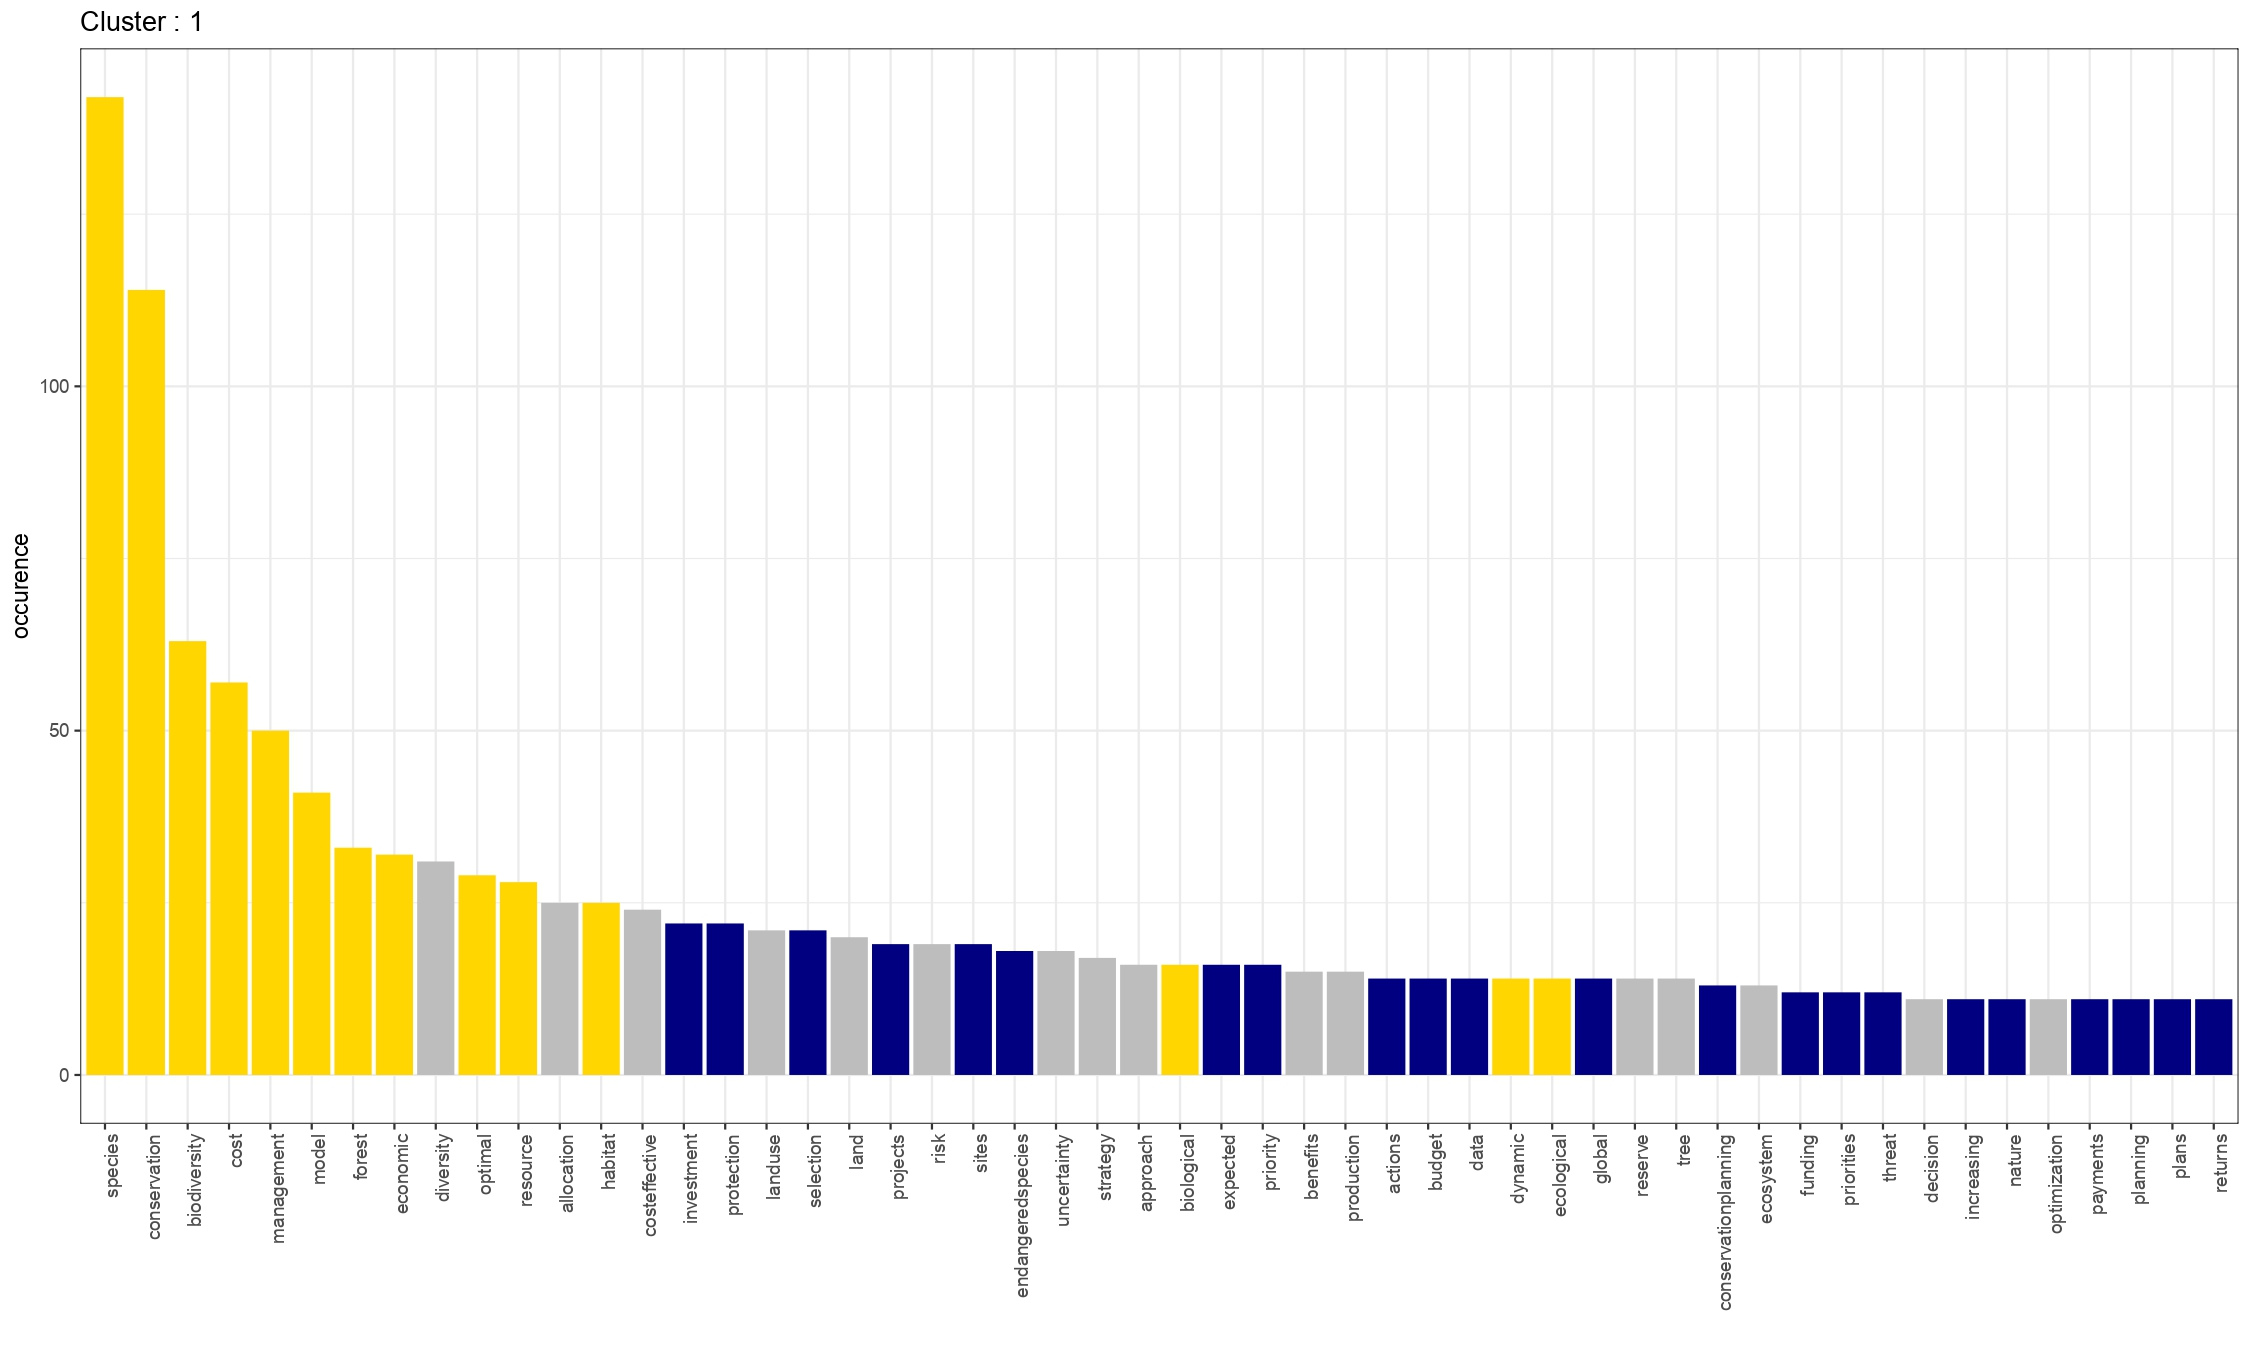
\includegraphics[width = .8\textwidth]{figures/review/occurence_kmodes_new_1_n50_common.png}\\
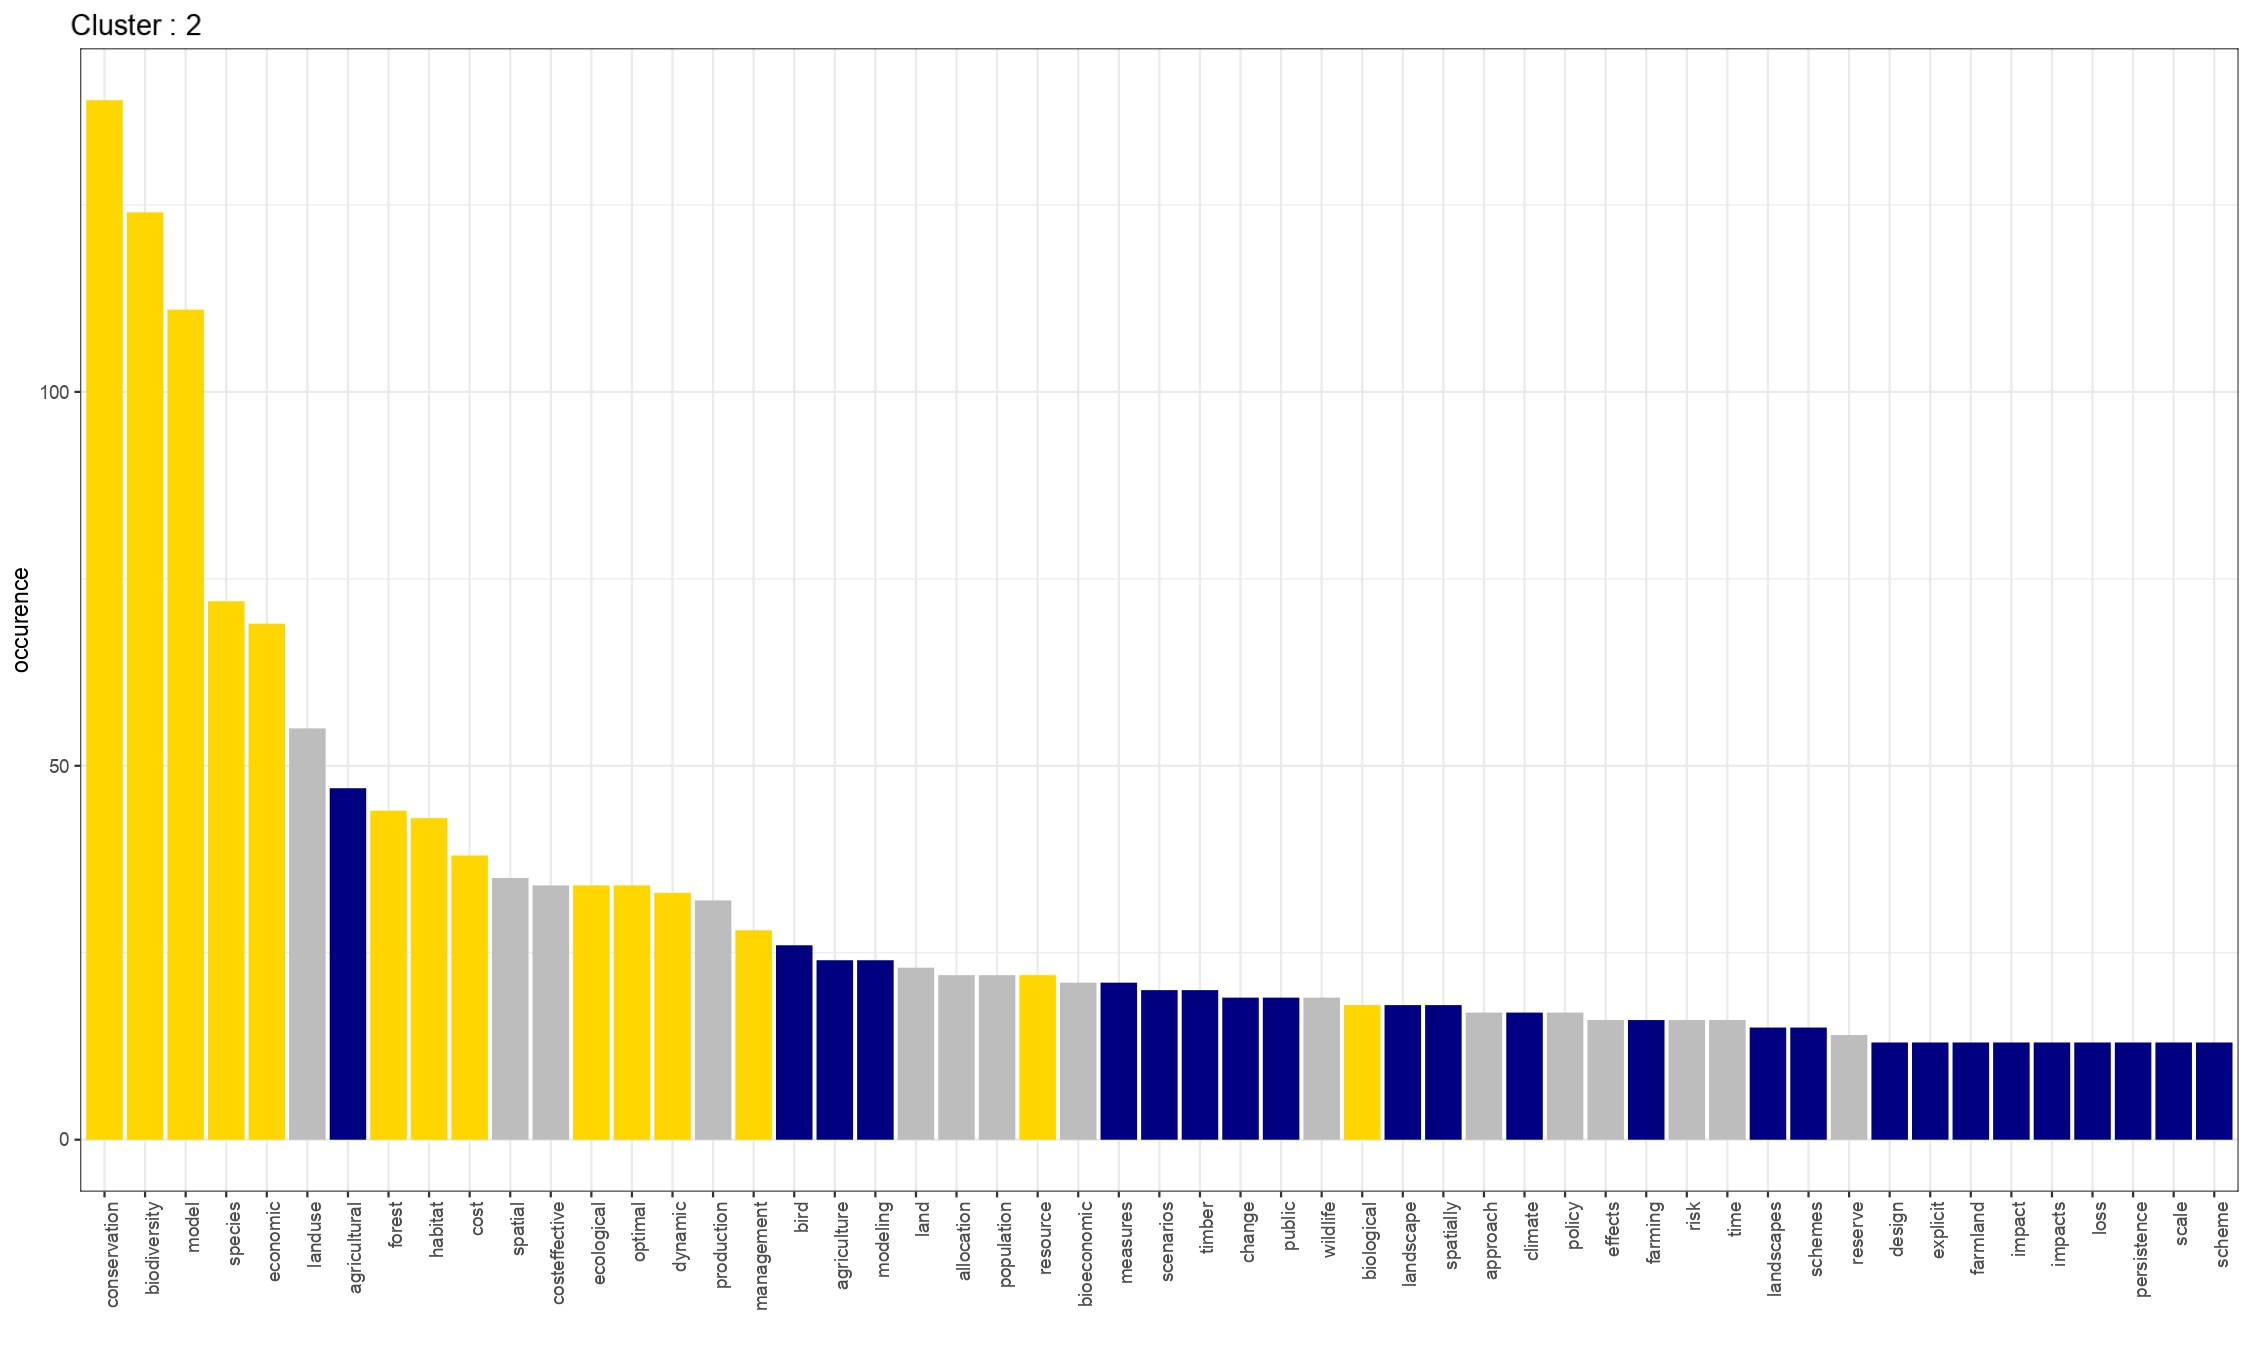
\includegraphics[width = .8\textwidth]{figures/review/occurence_kmodes_new_2_n50_common.png}
\caption{ Distribution profiles of the 50 words the more frequent for methodology-based groups 1 and 2}
\subcaption*{In yellow stand the words in common among the 4 profiles. On the opposite in blue stand the words specific to a profile}
\label{fig:words-profile-1}
\end{figure}

\begin{figure}[h]
\centering
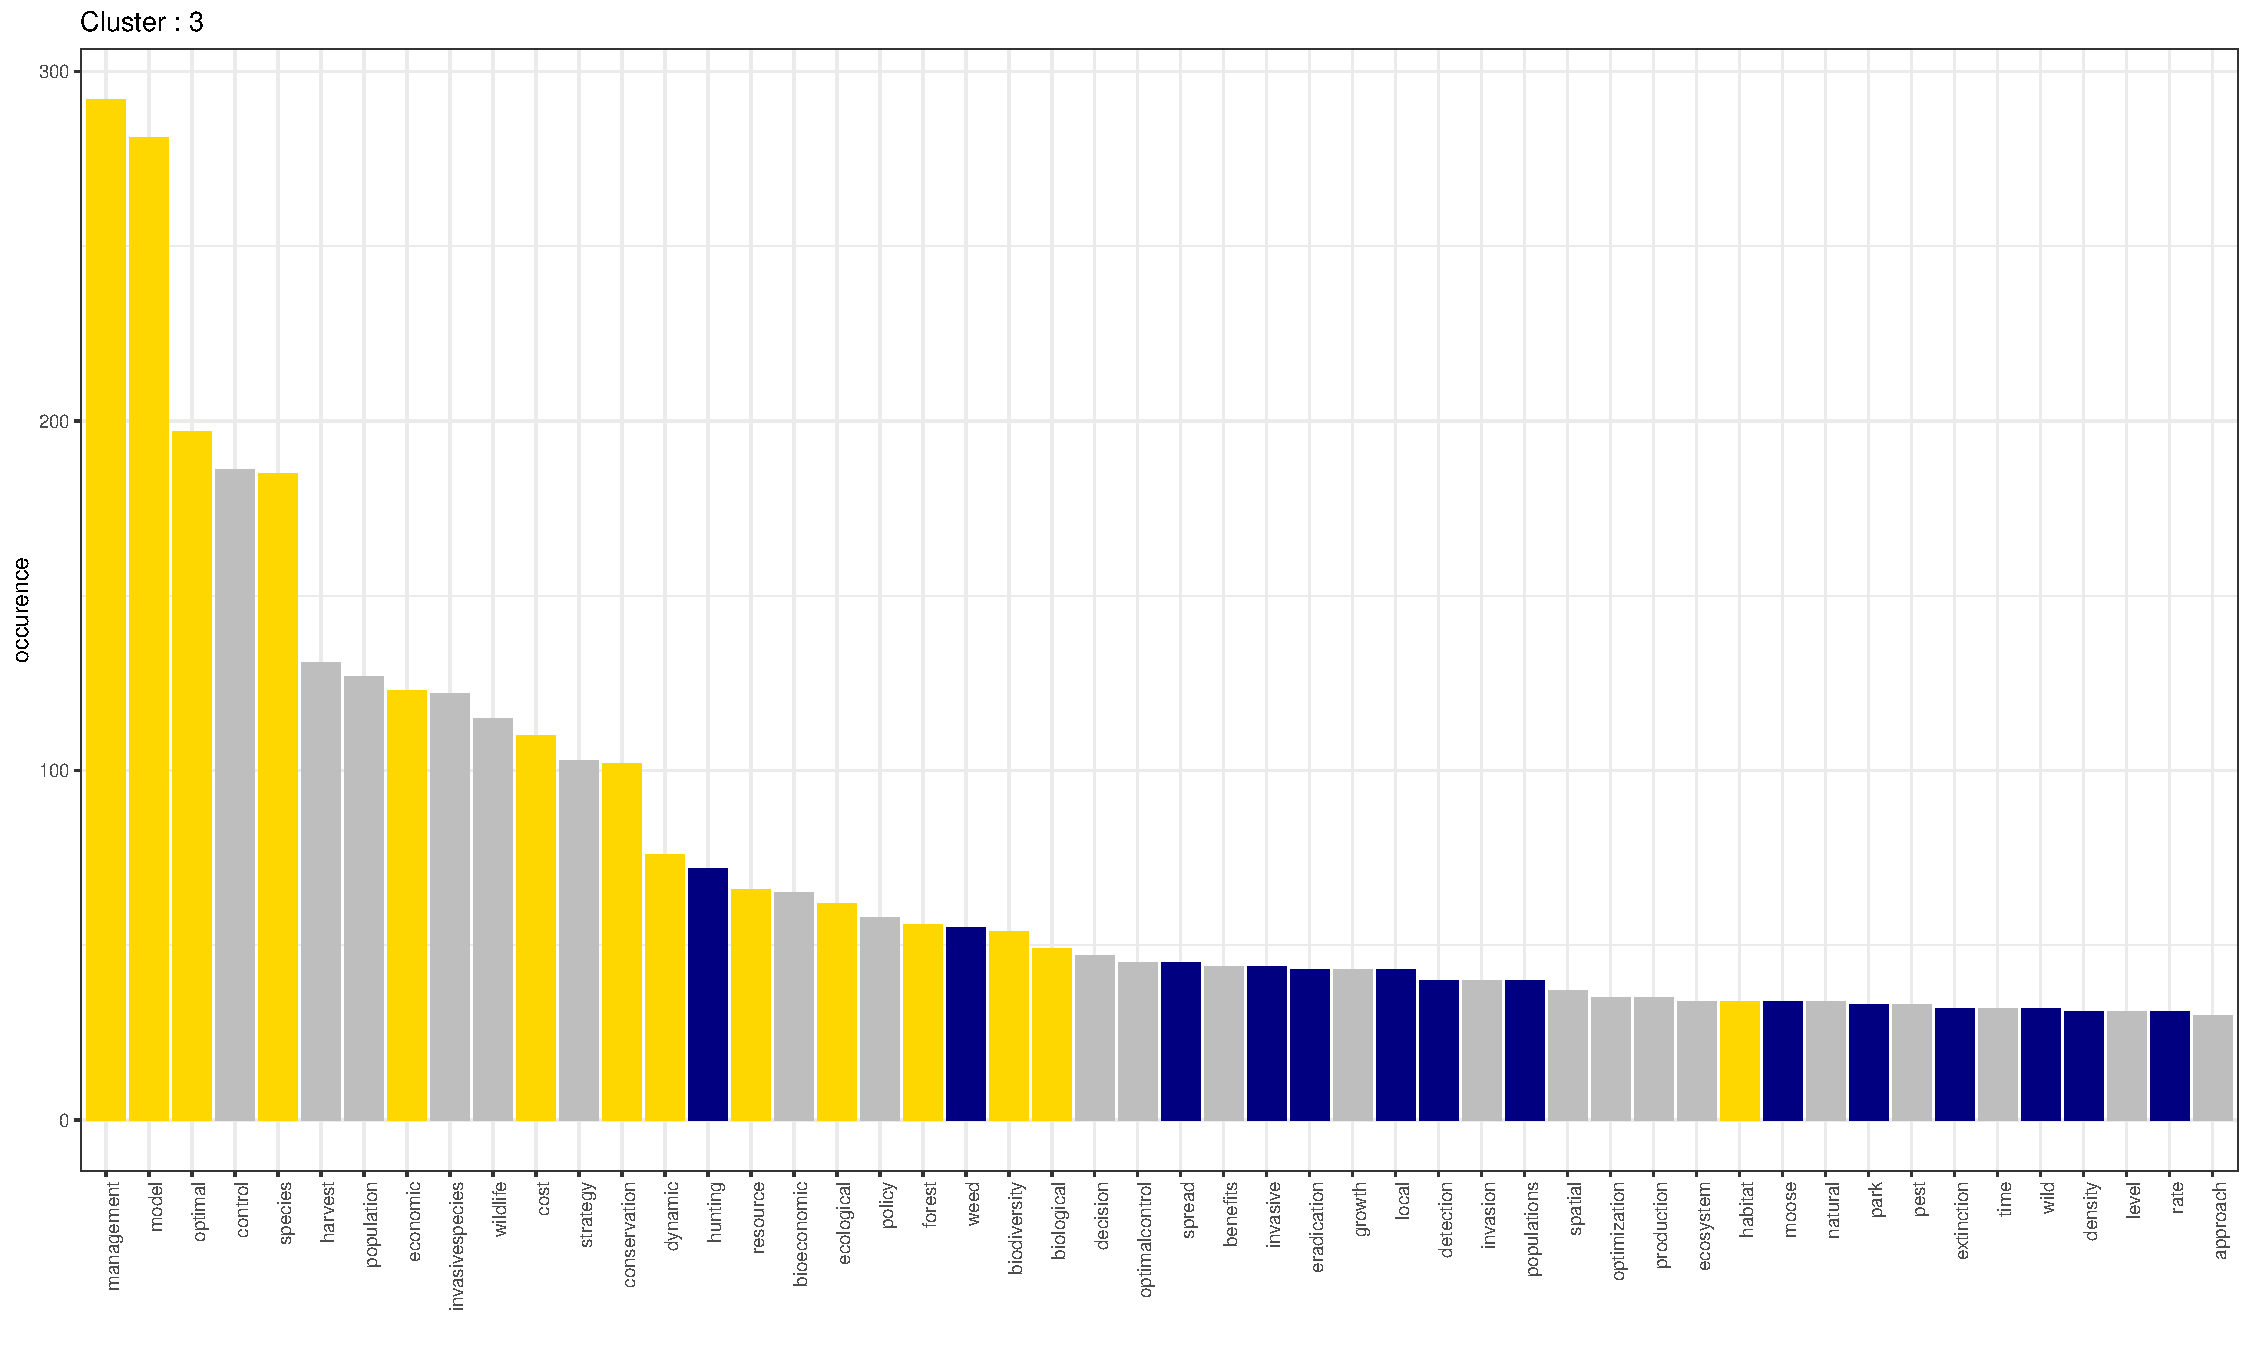
\includegraphics[width = .8\textwidth]{figures/review/occurence_kmodes_3_n50_common.pdf}\\
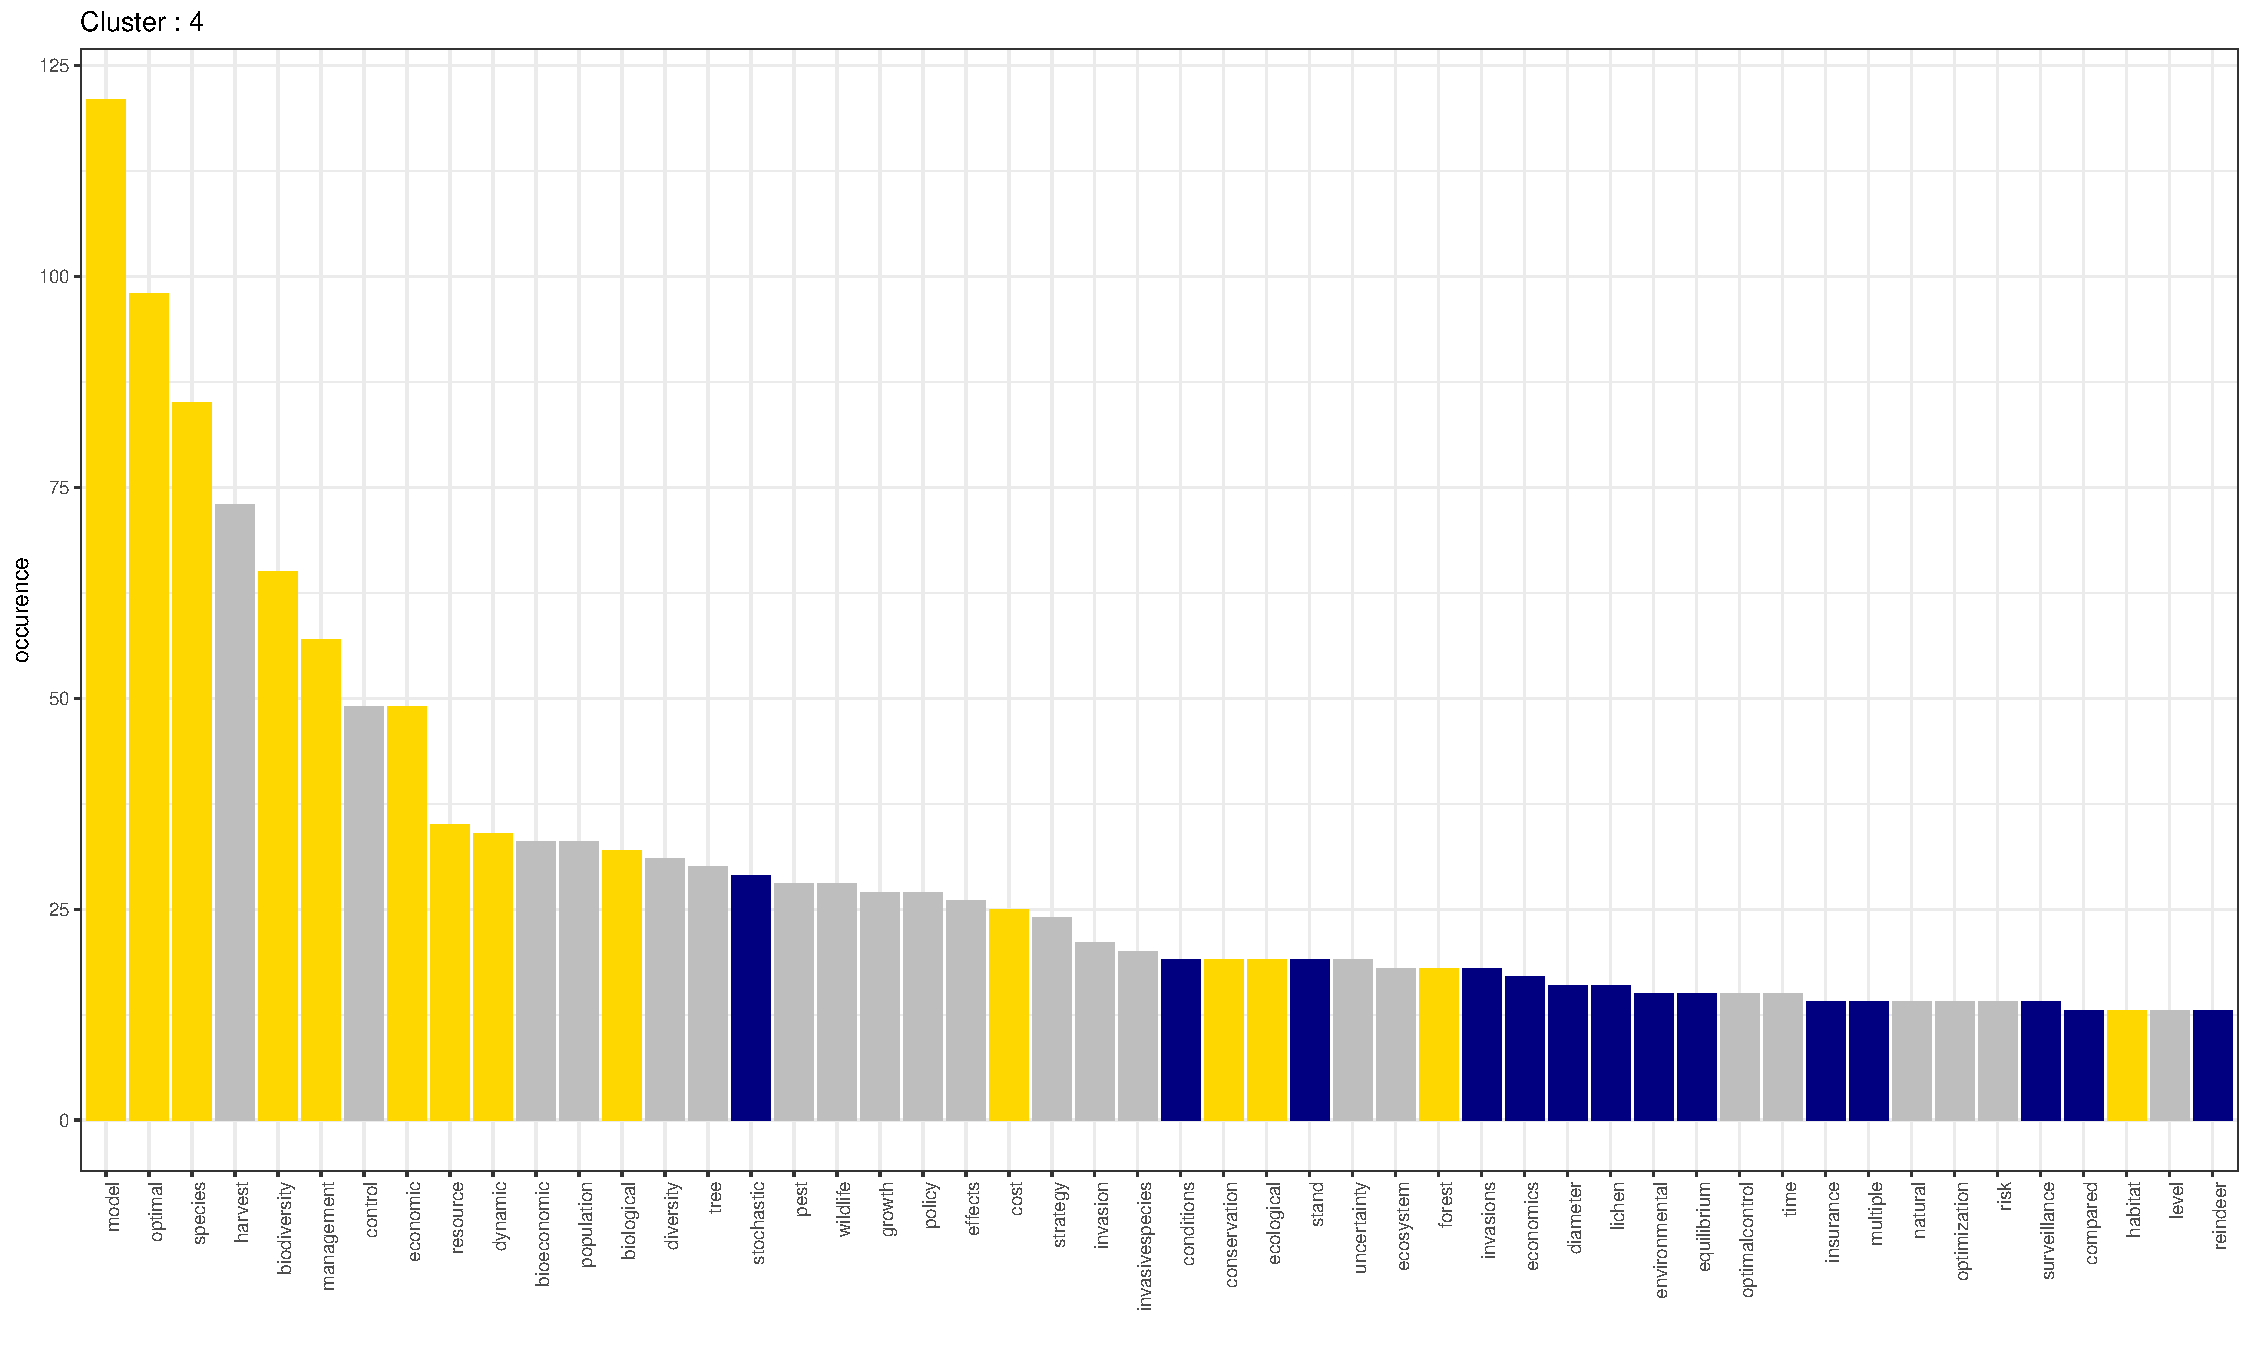
\includegraphics[width = .8\textwidth]{figures/review/occurence_kmodes_4_n50_common.pdf}\\
\caption{Distribution profiles of the 50 words the more frequent for methodology-based groups 3 and 4}
\subcaption*{In yellow stand the words in common among the 4 profiles. On the opposite in blue stand the words specific to a profile}
\label{fig:words-profile-2} 
\end{figure}

\begin{figure}[h]
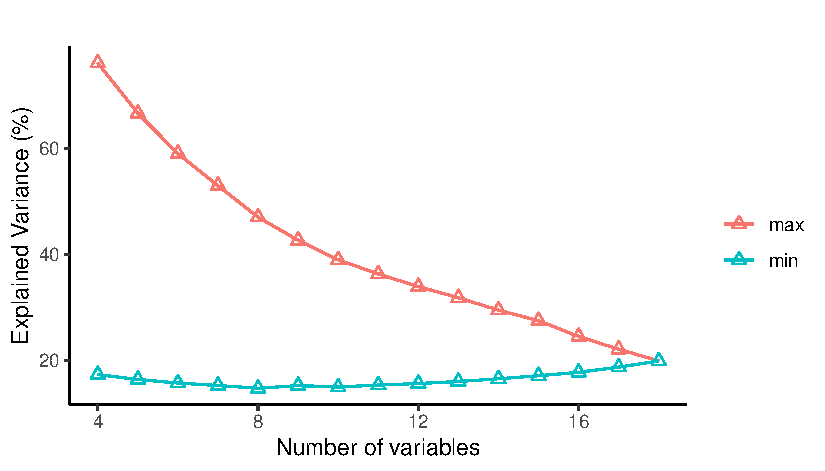
\includegraphics[width=.8\textwidth]{figures/review/variables_variance_enveloppe.pdf}
\caption{\label{fig:nb-crit-methodo} Explained variance function of the number of methodological criteria used in the MCA.}
\end{figure}

\begin{figure}[h]
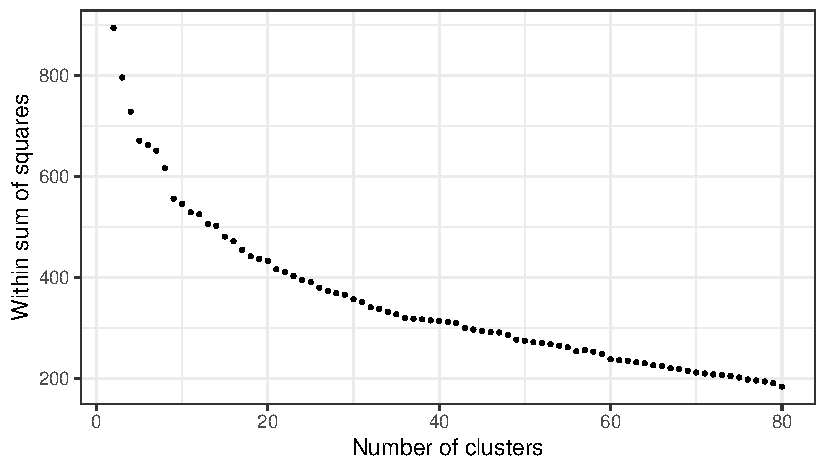
\includegraphics[width=.8\textwidth]{figures/review/kmodes_elbow.pdf}
\caption{\label{fig:cost-function} Cost function of the K-modes.}
\end{figure}

\begin{figure}[h]
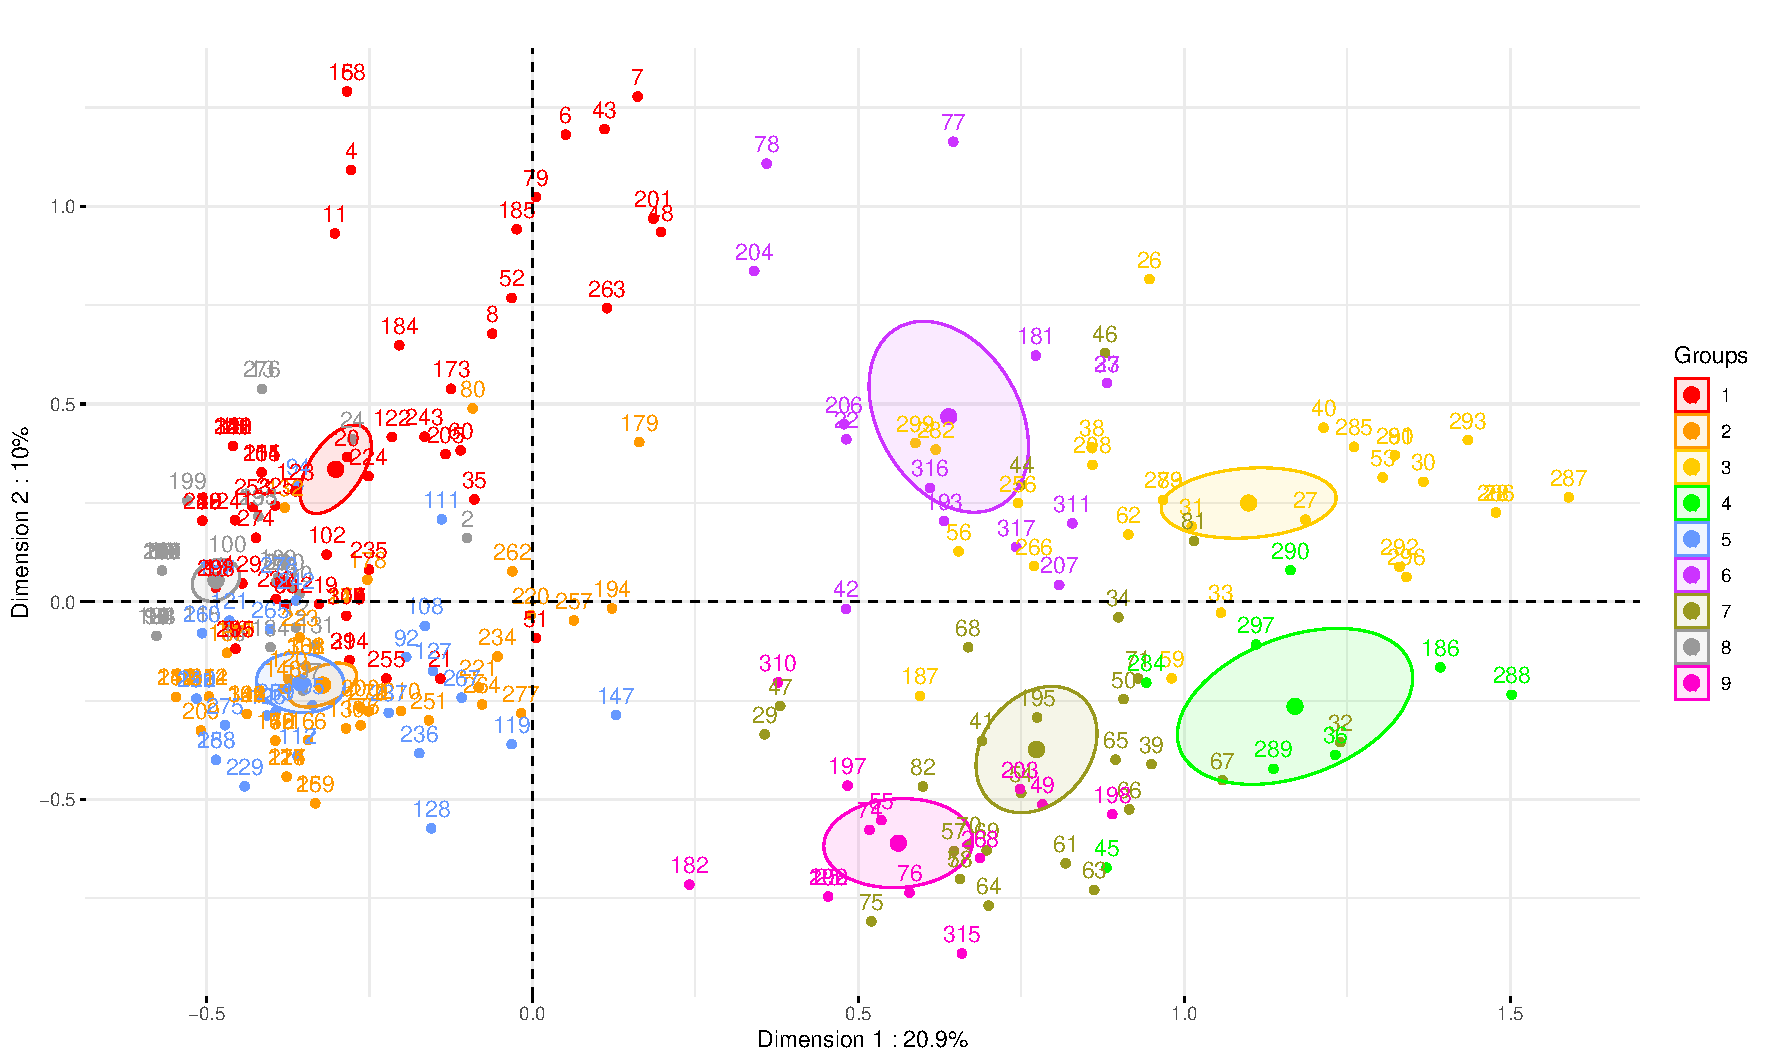
\includegraphics[width=.8\textwidth]{figures/review/mca_ind_automated_kmodes9.pdf}
\caption{\label{fig:MCA-9groups} Multiple Correspondence Analysis (MCA) running on 12 methodological criteria and 9 groups.}
\end{figure}